\chapter{Estado del arte}

\section{Introducción}
En este trabajo se presenta una técnica novedosa de transmisión de datos en redes de tipo broadcast de manera criptográficamente segura utilizando técnicas de espectro expandido.
Los sistemas de comunicaciones ópticos han echo posible las comunicaciones modernas, tecnologías como Internet comunicaciones celulares no son posibles sin una infraestructura optica de comunicaciones de alta velocidad.
Generalmente las redes de alta velocidad son switcheadas y sobre la capa física solo recientemente han sido utilizadas modulaciones y codificaciones mas complejas que un simple Xon-Xoff.
El Backbone ha evolucionado recientemente de 10Gbps, 100Gbps y 400Gbps al momento de escribir este documento, en donde se comienzan utilizan modulaciones de tipo WDM y modulación coherente [CITA]. Estas redes son generalmente switcheadas, en los que un ruteador central procesa electrónicamente los paquetes de datos y los retransmite a los nodos clientes por lo que es un canal dedicado.
Existen redes de tipo broadcast donde existen ventajas como un sistema de ruteo mucho mas simple que puede ser totalmente óptico, pero también poseen varios problemas como tener que compartir el ancho de banda, y problemas de seguridad inherentes al enviar la información a todos los nodos de la red. Este trabajo apunta a solucionar este ultimo problema utilizando tecnicas de tipo CDMA para la transmisión y un código corrector de errores que aprovecha la naturaleza asimétrica de la interferencia en fibra óptica.

\subsection{Códigos correctores de errores}
En toda comunicación es importante la confiabilidad de la misma, y como ningún sistema es perfecto es esperable que se produzcan errores en la transmisión que se presentan como bits erroneos detectados por el receptor. 
La manera mas simple de corregir estos errores es usar un algoritmo de detección de errores como puede ser un Checksum, CRC o hash[CITA], e iniciar un proceso de retransmisión de la porción o trama de datos afectada. Esto posee la desventaja de ser costoso tanto en t


\subsubsection{BCH-Reed Solomon}
\subsubsection{LDPC}
\subsubsection{Viterbi/Convolucional}

\subsection{Espectro ensanchado}
\label{espectroensanchado}
El espectro ensanchado, Spread Spectrum o CDMA es una técnica donde se utiliza mucho mas espectro del medio de transmisión que el necesario para la transmisión correcta de los datos.
Los origines datan del 1900, cuando Nicola Tesla patentó el concepto de \textit{"Frequency hopping"}.
El spreading de la señal tiene varias ventajas:
\begin{enumerate} 
\item Resistencia al espionaje, ya que solamente las partes que conocen la señal de spreading pueden decodificar la señal original
\item Resistencia contra interferencias de banda angosta (No a interferencias de banda ancha como el ruido térmico)
\item Capacidad de acceso múltiple. Varios usuario pueden transmitir en la misma frecuencia mientras utilicen diferentes códigos.
\end{enumerate} 
Adicionalmente, al guiarse la señal expandida con un generador pseudo-aleatorio o PRBS, se puede agregar privacidad a la comunicación haciendo imposible decodificar los datos sin tener los parámetros del PRBS.

A su vez, se puede expandir la señal en tres dominios:
\begin{enumerate} 
\item Direct Sequence (CDMA): Se expande la señal multiplicándola (XOR) con la señal de spreading, generalmente mucho más rápida. Este método es el utilizado en WiFi y WiMAX, redes 3G de celulares, etc.
\item Frecuency Hopping: La señal de spreading es utilizada para variar la frecuencia portadora de la señal original. Este método es utilizado por ejemplo en BlueTooth. (Se utiliza Adaptive Frequency Hopping, un método para evitar frecuencias con mucha interferencia)
\item Time Hopping: La señal de datos no transmite todo el tiempo, sino que sufre de un delay que depende de la señal de spreading. Este método no es muy utilizado aunque lo estudiaremos detenidamente en nuestro caso ya que es muy sencillo de implementar con los recursos de los que disponemos.
\end{enumerate} 


La desventaja del expectro expandido, que es utilizar mucho espectro por bits transmitido, o lo que tambien se denomina baja densidad espectral, a veces no afecta demasiado al tener el canal una cantidad disponible de espectro mucho mayor a la utilizada. Un ejemplo de un protocolo de comunicaciones que utiliza CDMA es el protocolo WIFI, en todas sus versiones.

\subsection{Códigos de generación pseudo-aleatorio}
Para que un codigo CDMA pueda utilizarse para obtener privacidad en la comunicacion, es necesario que el parametro a expandir, sea la frecuencia, el tiempo o el codigo utilizado, sea guiado o seleccionado por un generado pseudo-aleatorio o PRBS, que son algoritmos que basados en un parametro de inicializacion o semilla, son capaces de generar un stream de numeros aparentemente aleatorios, pero en realidad totalmente deterministicos. 
Es necesario que los nodos que participen de la comunicacion puedan generar exactamente la misma secuencia y compartan el parametro de generacion o semilla. Esto es equivalente a lo que en criptografia se denomina un algoritmo criptografico simétrico.
Existen muchas maneras y algoritmos de generar streams pseudo-aleatorios. Algunos algoritmos estan optimizados para que su periodo (la cantidad de numeros en su salida antes que el patron se repita) sea enorme, como por ejemplo el algoritmo Mersenne-twister.
Otro parametro deseable en un PRBS es su sencillez y rapidez. Un generadores PRBS muy popular se denomina Lineal Congruential Generator y solo precisa de dos operaciones, una multiplicacion y una suma.

Estos ejemplos carecen de una caracteristica fundamental requerida en nuestro sistema: Que no se puedan predecir. Esta simple caracteristica no es en realidad trivial ya que muchas tecnicas existen para inferir datos acerca del generador PRBS, lo que supondria una falla en la seguridad de un sistema basado en dicho generador. Para evitar estos problemas existen los llamados generadores PRBS criptograficamente seguros. Como ejemplo podemos nombrar a los generadores shrinking o self-shrinking.

\subsection{Seguridad}
La propuesta es utilizar un sistema de espectro expandido con el objetivo principal de lograr la privacidad del canal al nivel fisico.
Se fijaron los siguientes parametros de seguridad:

. El sistema debe proveer confidencialidad, integridad y autenticidad de los datos.
. El sistema debe ser seguro sin importar la cantidad de clientes existentes o los datos que transmiten
. Un atacante no debe poder identificar los datos de un cliente, aunque controle todos los demas nodos de la red.

Con estos parametros se busco el algoritmo CDMA adecuado. Las caracteristicas de un sistema optico hacen muy complejo el hardware requerido para lograr CDMA o Frequency-Hopping, pero implementar Time-hopping no presenta costo ni dificultad adicional, asi que este fue el seleccionado para la implementacion de seguridad.
Varios algoritmos de asignacion del time-slot fueron analizados. Se necesita que la salida de los mismos sean códigos ortogonales, o sea, deben poseer un generador capaz de crear streams pseudo-aleatorios que nunca coincidan para no generar colisiones entre los clientes. Esto no es trivial sin compartir algun tipo de información entre todos los clientes, lo que debilita la seguridad del sistema. Por ejemplo, codigos existentes llamados gold-codes permiten la generacion de multiples secuencias con baja cross-correlacion, muy util para coordinar dispositivos que comparten el medio. Pero desde el punto de vista de la seguridad, este codigo es trivialmente derrotado. Por ejemplo en un esquema donde un atacante controla todos los canales menos uno, el atacante podria simplemente dejar de transmitir y revelar la secuencia utilizada por la victima, que forzosamente estara utilizando el canal restante.

Se decidio por utilizar una codificacion trivial: Seleccionar el time-slot de acuerdo a una secuencia criptograficamente segura estandard, totalmente independiente de los otros nodos. Es demostrable que esta decision produce un sistema extremadamente simple y seguro. Como contrapartido, produce una cantidad muy elevada de colisiones que aumenta exponencialmente con el numero de clientes. Sin embargo, estas colisiones pueden ser corregidas mediante codificacion adicional, y se logro una utilizacion de canal muy cercana al maximo teorico como se demostrara en la proxima seccion. De echo, es en esta codificacion adicional donde reside el principal aporte de esta tesis.

\subsubsection{Security considerations and cypher strength}\label{security}
%% extraido de dline-pub.tex
There are several aspects of security to a communication channel: Authentication, reliability, confidentiality, and integrity.
The scheme presented in this paper uses CDMA to provide confidentiality, reliability, and integrity between two or more parties, and is equivalent to a shared-key symmetric encryption scheme where the shared key is used to initialise the PRNG.
Additional aspects like authentication can be implemented using logical-layer protocols.
We specifically designed the proposed system taking into consideration attacks of the sort presented in Ref. \cite{Shake:05}.

As system security relies on the strength of its PRNG, special care must be observed in the selection and implementation of a suitable cryptographically strong algorithm.
The proposed PRBS is non-linear, e.g., as in a self-shrinking generator~\cite{Meier:94}.
Additionally the user's key is never broadcast to the network, so key distribution must be performed beforehand using a secure channel.

We address an additional vulnerability inherent to optical systems arranged as a star network: CDMA algorithms depend on interference for confidentiality.
However, in an optical star-topology there are locations where little or no interference among users is present, for instance, next to the transmitter output of an end user the signal power is high and can be singled out from the background noise.
Note that even if the hypothetical eavesdropper can locate and observe the bits of the transmitted symbol, they cannot infer any information.
As positions within the data frame can overlap, the eavesdropper will observe a symbol with a HW between 1 and HW$\times$K, but it is not possible to reconstruct the right order of the bits without the PRNG seed.

Most encryption algorithms rely on XORing (the case of the RC4 encryption algorithm), a combination of substituting/scrambling of the bits before transmission (AES and DES encryption algorithms), or more complex transformations (RSA or Elliptic Curve algorithms), see Ref.~\cite{Menezes:1996:HAC:548089}.
However, these techniques necessarily modify the Hamming weight of every symbol in a way that is not optimal for our CDMA scheme as it increases intersymbol interference.
As the presented algorithm relies on time-hopping CDMA, it effectively encrypts symbols while maintaining the desirable low Hamming weight, increasing total bandwidth utilisation as shown in Fig.~\ref{fig_use}.

\begin{figure}[t]
  \centering
  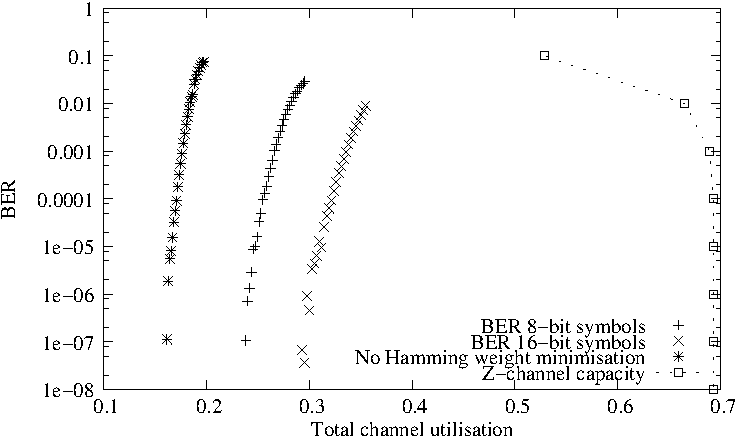
\includegraphics[width=0.48 \textwidth]{BERvsChannel} 
  \caption{Utilisation of the 10 Gbps channel. Each one of the 123 to 158 users transmitted 1 Gbit of data. Note the improvement in bandwidth utilisation compared to that in~\cite{ortega11}.}
  \label{fig_use}
\end{figure}

In contrast to TDMA, in our scheme the eavesdropper needs to intercept every optical fibre to reliably identify each end user as they are anonymised after passing through the central hub.
